\documentclass[12pt]{article}
\usepackage{somar}
\graphicspath{ {./img/} }

\title{Getting Started with SOMAR}
\author{Ed Santilli \& Alberto Scotti}
\date{\today}

%\author{Edward Santilli}
%\ead{santilli@physics.unc.edu}
%\address[Santilli]{Dept. of Physics, 214 Phillips Hall, UNC, Chapel Hill, NC 27599}
%\cortext[cor1]{Corresponding author}

%\author{Alberto Scotti}
%\ead{ascotti@unc.edu}
%\address[Scotti]{Dept. of Marine Sciences, 3117H Venable Hall, UNC, Chapel Hill, NC 27599}

 
\begin{document}
 
%\input{./tex/title.tex}
\maketitle
\tableofcontents
\newpage
%\listoffigures
%\listoftables
% 

\section{Introduction}

\subsection{Notation}\label{sec:notation}
\begin{itemize}
  \item $b_T$ = the total buoyancy (reduced gravity) field.
  \item $\bar{b} = \bar{b}(z)$ = the background buoyancy profile.
  \item $b$ = the buoyancy deviation.
  \item $u^\alpha$ = Cartesian component of the vector $\vec{u}$.
  \item $w$ = vertical Cartesian velocity component.
  \item $u^i$ = Curvilinear (mapped) component of the vector $\vec{u}$.
%  \item $u^{n,i}$ = $u^i$ at time $t^n$. $n$ will never be used as an index.
%  \item $u^{\star,i}$ = an unprojected velocity component.
%  \item $\uad^i$ = the time and face centered, projected advecting velocity.
%  \item $u_H^i$ = interpolation of $\uad^i$ to all cell faces.
  \item $\nu$, $\kappa$ = kinematic viscosity and scalar diffusion parameters.
  \item \{$x$, $y$, $z$\} or \{$x^\alpha$\} = Cartesian coordinates.
  \item \{$\xi$, $\eta$, $\zeta$\} or \{$\xi^i$\} = general curvilinear coordinates.
  \item $g_{i j}$, $g^{i j}$ = the metric tensor and its inverse.
  \item $J$ = $\sqrt{\left|\det(g_{ij})\right|}$ = $\det\left(\frac{\partial x^i}{\partial \xi^j}\right)$ = the Jacobian determinant.
%  \item CC = cell centered.
%  \item FC = face centered.
%  \item PPM = Piecewise parabolic method.
%  \item MAC = Marker-and-cell scheme that describes the exact, discrete projection method. \cite{HarlowWelch1965}
%  \item $\phi$ = scalar used during the MAC projection.
%  \item $\pi^l$ = pressure computed during the level $l$, CC velocity projection.
%  \item $\text{Av}^{\text{CC}\rightarrow\text{FC}}$ = averaging operator that sends CC data to FC data.
%  \item $\text{Av}^{\text{FC}\rightarrow\text{CC}}$ = averaging operator that sends FC data to CC data.
%  \item $\epsilon$ = average rate of dissipation of turbulence kinetic energy per unit mass.
%  \item $\epsilon_{ijk}$ = the totally anti-symmetric permutation symbol.
%  \item $\varepsilon_{ijk} = J \epsilon_{ijk}$ = the covariant
%Levi-Civita tensor.
  \item $\varepsilon_{ijk}$ = the covariant Levi-Civita tensor.
\end{itemize}


\subsection{Equations of Motion}\label{sec:eom}
We wish to calculate numerically the baroclinic response of a
stratified fluid 
of arbitrary depth to arbitrary forcing. To the extent that the barotropic
forcing is assumed as given, we assume that the fluid is capped by a rigid
lid. Future implementations will relax this assumption. 
Our main interest lies with geophysical flows as they occur in coastal
areas, which are characterized by the following properties: 
\begin{enumerate}
\item The density variation, $\Delta\rho/\rho_0$, within the fluid, 
normalized with a suitable 
characteristic density, $\rho_0$, is small.
\item The fluid velocity, $u$, is much smaller than the speed of sound, $c$. 
\item The extent of the vertical excursion engendered by the flow, $h$, is
  small relative to the vertical distance over which compressibility
  effects due to the increase of pressure become important, $c^2/g$. 
 \item The equation of state is linear and a single species (usually
  temperature) determines the density. Inclusion of second species (e.g.,
  salinity) is straightforward provided the equation of state remains linear. 
\item The horizontal to vertical dimensions ratio (aspect ratio) 
of the domain may be large, but we allow motion to occur on horizontal scales
that may be comparable or even smaller than the total depth. 
\end{enumerate}  
Under these conditions, the appropriate dynamic model is provided by the 
 Navier-Stokes equations in the Boussinesq approximation (NSE
from here on) \cite{Cushman1994} 
\begin{subequations}\label{NSE}\begin{align}
  &\dt{\vec{u}} = -\nabla\cdot\left(\vec{u} \vec{u}\right) - \nabla p +
    \nabla\cdot\tensorarrow{{\cal F}}_u - b_T \hat{z} + 2\vec{\Omega}\times\vec{u}+\vec{f}_\text{ext}, \\
  &\dt{b_T} = -\nabla \cdot \left( \vec{u} b_T \right) +\nabla\cdot\vec{\cal F}_b,\\
  &\nabla \cdot \vec{u} = 0.
\end{align}\end{subequations}
We define $b_T=g (\rho-\rho_0)/\rho_0$ as the reduced gravity, or buoyancy,
where $\rho_0$ is a representative density scale and $2\vec{\Omega}$ is the Coriolis parameter. Both $p$ and
$\vec{f}_\text{ext}$ are similarly defined as specific (per density) values of
pressure and body force.
The terms ${\tensorarrow{\cal F}}_u$ and ${\vec{\cal F}}_b$ represent  frictional and
diffusive effects respectively. For a Newtonian fluid,
\begin{subequations}
  \begin{equation}
    {\tensorarrow{\cal F}}_u = \nu \left( \nabla\vec{u}-(\nabla\vec{u})^T \right)
  \end{equation}
  and
  \begin{equation}
    {\vec{\cal F}}_b = \kappa \nabla b_T,
  \end{equation}
\end{subequations}
where
$\kappa$  is the diffusivity of the stratifying agent and $\nu$ the viscosity.
These terms become effective only  
at scales comparable or smaller than the Kolmogorov, $\eta_{\rm K}=\mathcal{O}(
\nu^{3/4}\epsilon^{-1/4})$, and Batchelor scales, $\eta_{\rm
  B}=\mathcal{O}(\eta_{\rm K}\kappa^{1/2}\nu^{-1/2})$, which in  typical 
geophysical conditions are $\mathcal{O}(1\rm{mm})$ or smaller. Therefore, in all
cases when 
the numerical grid is not fine enough to capture these scales, ${\tensorarrow{\cal{F}}}_u$ and $\vec{\cal F}_b$ need to be modified to include the effect of
the unresolved scales, either by increasing the value of the viscosity and
diffusivity above their molecular values (so called ``eddy'' viscosity and
diffusivity), or considering more sophisticated closure schemes. 
Since diffusive terms can
be included at little extra cost, even when viscosity and diffusivity are not
uniform, we retain them.\\

Note that the body force is made up of the sum of the gravitational term,
$b_T\hat{z}$, and a generic body force which may include the effect of barotropic forcing (surface tide). The reason for the
split will become clear in the following.\\

In geophysical applications, the fluid is generally stably stratified, at least
over  sufficiently large scales. 
It is thus advantageous to split the buoyancy into a
background and deviation, 
\begin{equation*}
	b_T(\vec{x},t) = \bar{b}(z) + b(\vec{x},t),
\end{equation*}
where $\bar{b}(z)$ is chosen to describe the static vertical profile of the
fluid. The equations of motion now become
\begin{subequations}\label{BVNSE}
  \begin{align}
    &\dt{\vec{u}} = -\nabla\cdot\left(\vec{u} \vec{u}\right) - \nabla p +
      \nabla\cdot{\nu\nabla\vec{u}} - b\hat{z} + 2\vec{\Omega}\times\vec{u} + \vec{f}_\text{ext}, \\
    &\dt{b} = N^2 w -\nabla \cdot \left( \vec{u} b \right) + \nabla\cdot\kappa\nabla b,\\
    &\nabla \cdot \vec{u} = 0,
  \end{align}
\end{subequations} 
where the Brunt-V\"ais\"al\"a (BV) frequency is defined as $N^2=-d\bar{b}/dz$ and the background buoyancy forcing term has been swept into the pressure field. 
By solving for the fluctuations, $b$, rather than the whole field, $b_T$,
 we avoid diffusion of the background stratification and
allow for a special treatment of the stiff forcing terms.  There is a further reason for the
split. A stably stratified fluid supports internal waves, which propagate with
speeds that can be  larger than the physical fluid velocity.  Separating the mean stratification from the
fluctuations allows us to deal with  the corresponding hyperbolic problem with
an appropriate time integration scheme which is unconditionally stable.   
Setting $N=0$
recovers the original set of equations.
\\

%To accommodate complex topography, 
%we wish to write the NSE in a general curvilinear coordinate
%system. There are many ways to do this, but we choose a form that simplifies
%discretization and avoids connection coefficients.
To accommodate complex topography, we write the NSE in a general curvilinear coordinate system. One form that simplifies
discretization and avoids connection coefficients is
\begin{subequations}\label{GCNSE}\begin{align}
  &\dt{u^\alpha} = -\frac{1}{J}\partial_j Ju^j u^\alpha - g^{\alpha i}\partial_i p + \nu\nabla^2 u^\alpha - b\hat{z}^\alpha + 2{\varepsilon^{\alpha}}_{i j} \Omega^i u^j + f^\alpha_\text{ext}, \\
  &\dt{b} = \left[ N^2 w - \frac{1}{J}\partial_i J u^i b \right] + \kappa\nabla^2 b,\\
  &\partial_i J u^i = 0.
\end{align}\end{subequations}
The terms in square brackets are analytically identical to
$\nabla \cdot (\vec{u} b_T)$, the divergence of all scalar advective fluxes. In this paper, the symbol $w$ will always refer to the vertical Cartesian
velocity component. We use Latin indices to indicate tensor components
in the curvilinear basis while Greek indices refer to components in the Cartesian basis. For
example, $g^{\alpha j} = \jac{\alpha}{i} g^{ij}$ by definition. (See section
\ref{sec:notation} for a more complete description of the notation used in
this document.) The symbol $\nabla^2=J^{-1}\partial_i J g^{ij}\partial_j$ is
the Laplace-Beltrami operator. 
\\


\section{Requirements and compilation details}
This software uses the Chombo library\footnote{Chombo has been developed and is being distributed by the Applied Numerical Algorithms Group of Lawrence Berkeley National Lab.}, which in turn uses the HDF5 library \cite{hdf5}. (If you plan to compute in parallel, MPI-2 compliant software must also be installed.) When installing the HDF5 libraries, be sure to use version 1.6.9 and compile with the \texttt{--enable-production} configuration option. Listings \ref{lstHDF5serial} and \ref{lstHDF5parallel} provide examples of how to compile and install the HDF5 library for Chombo. In these listings, \texttt{\$\{ROOT\_DIR\}} can be replaced with your folder of choice.

\begin{lstlisting}[language=sh,caption={Serial HDF5 compilation example.},label=lstHDF5serial]
$ make clean
$ export FC=ifort; export CC=icc; export CXX=icpc
$ ./configure --prefix=${ROOT_DIR}/hdf5/serial --enable-production
$ make all
$ make install
\end{lstlisting}

\begin{lstlisting}[language=sh,caption={Parallel HDF5 compilation example.},label=lstHDF5parallel]
$ make clean
$ export FC=ifort; export CC=mpicc; export CXX=mpicxx
$ ./configure --prefix=${ROOT_DIR}/hdf5/serial --enable-production --enable-parallel
$ make all
$ make install
\end{lstlisting}

With HDF5 installed, you are ready to compile Chombo. Go to the \texttt{\$\{CHOMBO\_DIR\}/lib/mk} directory and copy \texttt{Make.defs.local.template} to \texttt{Make.defs.local}. This will create the main makefile that you must edit. This file is well commented and documented in both the ``Chombo Design Document'' and ``Chombo Makefile User’s Guide.'' To build the libraries, go to the \texttt{\$\{CHOMBO\_DIR\}/lib} directory and type \texttt{make lib}. If the compilation fails, try the following.
\begin{itemize}
  \item {Do not use \texttt{make all} to compile the Chombo libraries -- use \texttt{make lib}.}
  \item {Set \texttt{USE\_EB = FALSE}. We will not need the embedded boundary library.}
  \item {Set \texttt{USE\_MT = TRUE}. Turning the memory tracking feature off produces buggy code.}
  \item {If you are using the Intel compilers, try adding the \texttt{-lifcore} switch to \texttt{syslibflags}.}
\end{itemize}

Upon successful completion, at least 5 static libraries should be created: basetools, boxtools, amrtools, amrtimedependent, and amrelliptic. It will then be time to compile our AMR Navier-Stokes solver. Go to the project's \texttt{exec} folder and run \texttt{make all}. If the compilation fails, try the following.
\begin{itemize}
  \item {Try adding \texttt{-I\$\{MPI\_DIR\}/include} to \texttt{fdbgflags} and \texttt{foptflags}.}
  \item {Try adding \texttt{-llapack} to \texttt{syslibflags}.}
  \item {Try adding \texttt{-L\$(FFTW\_DIR)/lib -ldfftw -ldrfftw} to \texttt{syslibflags}.}
\end{itemize}


\section{Running a packaged simulation}
Before creating your own simulation, you should successfully test one of the packaged simulations that come with the solver. In the \texttt{exec} folder, you will see several input files. Each of these input files are targeted to run a specific problem on a specific machine and are identified accordingly (\texttt{inputs.problem.machine}). Suppose we want to run the lock exchange problem on a machine called HAL. As a rule, an input file for machine A should never be altered to work on machine B, so we should first copy one of the lock exchange input files to \texttt{inputs.LockExchange.HAL}.\\

Open this new file and look for the following lines (it's okay if some of them are missing).
\begin{lstlisting}
  # amr.restart_file = chkpt_000010.2d.hdf5
  # plot.plot_prefix = plot_             # [plot_]
  # plot.checkpoint_prefix = chkpt_      # [chkpt_]
  # plot.plot_period = 0.1
  plot.plot_interval = 1
  plot.checkpoint_interval = 100
\end{lstlisting}
In this listing, several of the lines are commented out with a \texttt{\#}. This usually means we do not want a particular feature turned on or we are happy with the default values. In this case, we do not want to restart a simulation from a saved state and we are happy with the default file name prefixes. Whenever a feature has a default value, it will be shown on the right in square brackets. As you can see, all plot files will be prefixed with \texttt{plot\_} and all checkpoint files (files used to restart the simulation) will be prefixed with \texttt{chkpt\_}. If we want the plot files to go into a different directory, we can uncomment the plot\_prefix line to read \texttt{plot.plot\_prefix = /home/user/myPlotFolder/plot\_}. Other input parameters such as \texttt{amr.final} and \texttt{amr.maxsteps} can be altered as you see fit.\\

%TODO
%For a complete list of input parameters, see section \hilight{???}.\\

Now it is time to compile a 2D simulation with debugging off. Make sure that the Chombo makefile \texttt{Chombo/lib/mk/Make.defs.local} knows this before running make.
\begin{lstlisting}
  DIM   = 2
  DEBUG = FALSE
  OPT   = HIGH
\end{lstlisting}
Next, run \texttt{make all} from the \texttt{exec} directory. This will create an executable with an \texttt{OPTHIGH.MPI.ex} suffix. This executable must be given an input file as a parameter. For example, to run a simulation on 8 processors, use \texttt{mpirun -np 8 somar2d.OPTHIGH.MPI.ex inputs.LockExchange.HAL}. The result should be two sets of HDF5 files -- one set of checkpoint files that are used to restart a simulation, and one set of plot files that can be viewed in VisIt\footnote{VisIt is freely available at \url{https://wci.llnl.gov/simulation/computer-codes/visit}.}.\\

In the interest of efficiency, be sure to set the \texttt{amr.max\_base\_grid\_size} input parameter to be commensurate with \texttt{amr.nx}, and yet be large enough for the multigrid solver to be effective. It is also wise to ensure that the total number of grids is a multiple of the number of processors. If you neglect to add a \texttt{amr.max\_base\_grid\_size} line to your input file, the solver will try to decompose the domain automatically, but it does not always do a perfect job. It's best to get into the habit of manually setting the \texttt{amr.max\_base\_grid\_size} and checking it each time you change the problem setup.\\

To add AMR features, consider the input parameters shown in listing \ref{lstRegriddingParams}. Setting \texttt{maxlevel=1} will give us the base level ($0$) and a single refined level ($1$). When AMR is turned on, we must supply \texttt{regrid\_intervals} and \texttt{refratio} values. (For the sake of brevity, I will not write input prefixes every time I reference a parameter.)
\begin{lstlisting}[caption={The regridding input parameters.},label=lstRegriddingParams]
  amr.maxlevel = 1
  amr.regrid_intervals = 4 4 4
  amr.refratio = 4 1
  # amr.tags_grow = 1
  # amr.vel_tag_tol = 0.4
  # amr.buoyancy_tag_tol = 0.4
  amr.magvort_tag_quota = 0.125
  # amr.vort_tag_tol = 0.0 0.0 0.01
\end{lstlisting}

The \texttt{regrid\_intervals} parameter is a vector of integers specifying how many timesteps must pass before a level is tagged for refinement. For example, suppose we set \texttt{maxlevel=2} and \texttt{regrid\_intervals=1 2 4 3 7}, then level 0 will be tagged for refinement at every level 0 timestep, level 1 will be tagged every other level 1 timestep, and level 2 will never be tagged since we are not allowing a finer level. The last three vector elements of \texttt{regrid\_intervals} are unnecessary and will be ignored by the solver. There is a compromise that must be made when setting these values. If you increase this interval, the solver will regrid less often. On one hand, this is good because regridding is expensive. On the other hand, this is bad because the grids may not adapt quick enough to keep up with important advecting features. \\

The \texttt{refratio} parameter is a vector with \texttt{SpaceDim}\footnote{Chombo defines the integer constant \texttt{SpaceDim} to equal the number of spacial dimensions, as the name suggests. In C++ code, either \texttt{SpaceDim} or the macro \texttt{CH\_SPACEDIM} can be used. In Fortran, only \texttt{CH\_SPACEDIM} is available. See the Chombo Design Document for further details.} components. In this example, all levels will have a $\Delta x$ that is four times smaller than the next coarser level, while the vertical grid spacing remains unchanged. If you need more control over the refinement, it is possible to assign different refinement ratios to each level. If we add \texttt{refratio\_lev3 = 2 4} to the input file, then all levels will be refined according to the basic \texttt{refratio} prescription except level 3, which will use it's own, special
refinement ratio.\\

Both \texttt{vel\_tag\_tol} and \texttt{buoyancy\_tag\_tol} work in the same way. The relevant variables are scanned for large undivided differences. If, say, the buoyancy has two neighboring cells whose absolute difference is greater than the tagging tolerance, both cells are tagged for refinement. \texttt{magvort\_tag\_quota} works a bit differently. Cells are tagged when $|\vec{\omega}|$ is greater than this factor times $\max_{\vec{x}}|\vec{\omega}|$. Notice that \texttt{magvort\_tag\_quota} always results in tagged cells, which is why it is a quota. Finally, we have \texttt{vort\_tag\_tol}, which is always a three-dimensional vector. Cells will be tagged if $|\omega_d \, \Delta A_d| > \texttt{vort\_tag\_tol}_d$. In 2D, only the last component is used while in 3D, all components are used. None of these tagging strategies are universal. For each new problem, it is probably best to consider what the tagging criteria should be and create new code as needed. But that process lies outside of the scope of this introductory section.\\

The last input parameter we will discuss is \texttt{tags\_grow}. Once all cells on a level are tagged for refinement, it is often desirable to create a layer of additional tagged cells around the original tags. This will increase the number of points on the finer level, but provides a buffer zone to allow the resolved features to evolve without falling off the refined grids. This parameter should be set in tandem with \texttt{regrid\_intervals}. Typically, if I set \texttt{regrid\_intervals} to a large value, I offset the danger with a \texttt{tags\_grow} of $1$ or $2$. Setting this value wisely will also provide some flexibility when choosing tag tolerances.

\section{Creating a new simulation}
When you decide to create your own simulation, be sure that you are prepared to make extensive use of the BoxTools library. This is the component of Chombo that manages data over decomposed grids. In particular, chapter 2 of the Chombo Design Document should be well understood before attempting to write any C++ code. In this section, and in what follows, it will be assumed that you are fluent in C++ and are familiar with the BoxTools class structure. Additionally, if you plan to browse the AMR code, it would also be helpful to skim the chapter discussing "Chombo Fortran." This is Fortran 77 precompiled with the C preprocessor and a perl preprocessor in order to add features.\\

When creating a new simulation, there are typically three components that need to be understood:
\begin{enumerate}
  \item \textit{The input file} -- We've briefly discussed input files in the last section. They allow simulation parameters to be changed without recompiling. These parameters include the domain lengths, cell sizes, sponge strength, number of refinement levels, output file locations, and so forth. This file can be saved with the results to ensure reproducibility.
  \item \textit{The initial and boundary condition (IBC) tools} -- This component not only sets the IBCs, but also generates the sponge forcing terms, fixes the constant background buoyancy field, and optionally computes a restriction on the timestep due to the boundary layer.
  \item \textit{The geometry tools} -- This is the component that maps the physical coordinates to a set of curvilinear coordinates. Typically, this is used to produce terrain--following coordinates and to apply grid stretching near solid boundaries.
\end{enumerate}
We will explain the details of these three components as we step through the creation of a simple internal wave simulation. As before, make a copy of the \texttt{inputs.template.machine} file. To comply with the current naming scheme, name your new copy \texttt{inputs.InternalWave.machine}, where machine is replaced with the target computer name.\\

\subsection{Setting the initial and boundary conditions}\label{NewIBCSetup}
This is the first step, and unfortunately, it's also the most involved. We need to create our own boundary condition class, which means there is some C++ style overhead incurred during problem creation. This initial overhead, however, will be offset by the fact that we are creating a class that overrides a parent class. Most of the features we will ever need (e.g. solid wall boundary conditions, sponges, tidal forcing, splitting of the buoyancy into background and deviation, etc\dots) already exist in the parent, which means these features virtually come at no additional cost.\\

If you open \texttt{BCUtil/PhysBCUtil.H}, you can browse the functionality assigned to the IBC classes. While looking at this file, don't be nervous -- \texttt{PhysBCUtil} is the parent class of all problem-specific IBC classes. It contains a large amount of code to relieve its children's burden. We will be creating a child class called \texttt{InternalWaveBCUtil}. In order to compile, the absolute minimum this class must provide is a constructor and a \texttt{newPhysBCUtil} function. If we want this class to do anything interesting, we must also provide a \texttt{setScalarIC} function. Three functions -- that's it. A sample is provided in listings \ref{lstIWBCUtil.H} and \ref{lstIWBCUtil.cpp}.
\begin{lstlisting}[caption={The \texttt{InternalWaveBCUtil.H} file.}, label=lstIWBCUtil.H]
/*************************************************************************
 *    FILE: InternalWaveBCUtil.H
 *    DESC: Simple internal wave demo.
 *    DATE: Mon 13 May 2013 01:10:23 AM EDT
 *    MAIL: santilli@physics.unc.edu
 ************************************************************************/

#ifndef __InternalWaveBCUtil_H__INCLUDED__
#define __InternalWaveBCUtil_H__INCLUDED__

#include "PhysBCUtil.H"


class InternalWaveBCUtil: public PhysBCUtil
{
public:

    // Default constructor
    InternalWaveBCUtil ();

    // Factory
    virtual PhysBCUtil* newPhysBCUtil () const;

    // Fills a FAB with the initial scalars
    virtual void setScalarIC (FArrayBox&           a_scalarFAB,
                              const int            a_scalarComp,
                              const LevelGeometry& a_levGeo,
                              const DataIndex&     a_di) const;
};


#endif //!__InternalWaveBCUtil_H__INCLUDED__
\end{lstlisting}

\begin{lstlisting}[caption={The \texttt{InternalWaveBCUtil.cpp} file.}, label=lstIWBCUtil.cpp]
#include "InternalWaveBCUtil.H"

// -----------------------------------------------------------------------
// Constructor
// We don't need to do anything!
// -----------------------------------------------------------------------
InternalWaveBCUtil::InternalWaveBCUtil ()
{;}


// -----------------------------------------------------------------------
// Factory
// All this function does is create a new BC object for the AMR solver.
// Since the AMR solver needs to work with any child of PhysBCUtil,
// it is up to this function to define any problem-specific variables
// and then hand over a down-casted pointer.
// -----------------------------------------------------------------------
PhysBCUtil* InternalWaveBCUtil::newPhysBCUtil () const
{
    PhysBCUtil* newBCPtr = new InternalWaveBCUtil();
    return newBCPtr;
}


// -----------------------------------------------------------------------
// Fills an FArrayBox with the initial scalars.
// This is just about the simplest way you can set this problem up.
// We will do something more sophisticated later.
// -----------------------------------------------------------------------
void InternalWaveBCUtil::setScalarIC (FArrayBox&           a_scalarFAB,
                                      const int            a_scalarComp,
                                      const LevelGeometry& a_levGeo,
                                      const DataIndex&     a_di) const
{
	// Get a box that represents the entire domain from the LevelGeometry
	// class. Remember, a_scalarFAB may not be defined over the entire
	// domain because we have decomposed the domain.
	const Box& domBox = a_levGeo.getDomain().domainBox();

	// The plan is to cut the domain in half. The upper half will have
	// light fluid, and the lower half will have heavy fluid.
	int chopPoint = domBox.smallEnd(SpaceDim-1)
	              + domBox.size(SpaceDim-1) / 2;
	Box loBox = domBox;
	Box hiBox = loBox.chop(SpaceDim-1, chopPoint);

	// Now, we need to create the mixed region. You can adjust the size
	// of this region as you see fit.
	chopPoint = domBox.bigEnd(0) - domBox.size(0) / 30;
	Box mixedBox = domBox;
	mixedBox = mixedBox.chop(0, chopPoint);

	// Make sure these boxes lie within the definition of a_scalarFAB.
    loBox &= a_scalarFAB.box();
    hiBox &= a_scalarFAB.box();
    mixedBox &= a_scalarFAB.box();

    // Set the values!
    if (!loBox.isEmpty()) {
        a_scalarFAB.setVal(0.5, loBox, a_scalarComp);
    }
    if (!hiBox.isEmpty()) {
        a_scalarFAB.setVal(-0.5, hiBox, a_scalarComp);
    }
    if (!mixedBox.isEmpty()) {
        a_scalarFAB.setVal(0.0, mixedBox, a_scalarComp);
    }
}
\end{lstlisting}

Once this class is written, we need to register it with the list of problem types. This is done in two steps. First, open \texttt{util/ProblemContext.H} and look for a enumeration called \texttt{ProblemType}. Add a new entry to this list called \texttt{INTERNAL\_WAVE}. It is important that you do not alter any of the other entries or you will cause other problems to stop working. Next, open the associated .cpp file, \texttt{util/ProblemContext.cpp}, and go to the \texttt{newPhysBCUtil} function. This function contains a switch block that associates each problem with its appropriate boundary conditions. You must add your new \texttt{PhysBCUtil} to this list of cases.
\begin{lstlisting}[caption={The \texttt{ProblemContext} enumeration.},label=lstPhysBCUtilEnumerations]
    enum ProblemType {
        ADVECTION_TEST  = 0,
        LOCK_EXCHANGE   = 1,
        BEAM_GENERATION = 2,
        TAYLOR_GREEN    = 3,
        SOLITARY_WAVE   = 4,
        INTERNAL_WAVE   = 5,  // This is our new addition.
        _NUM_PROBLEM_TYPES
    };
\end{lstlisting}
\begin{lstlisting}[caption={The new addition to the \texttt{ProblemContext::newPhysBCUtil} switch block.}]
    case ProblemContext::INTERNAL_WAVE:
        physBCPtr = new InternalWaveBCUtil;
        break;
\end{lstlisting}

At this point, all of the code is in place. Now, we go to our input file and set \texttt{ibc.problem} equal to the number assigned in the enumeration. In the code of listing \ref{lstPhysBCUtilEnumerations}, \texttt{INTERNAL\_WAVE} was assigned the number $5$, but your code may be different. When the code runs, \texttt{ProblemContext} will read the input file, including the \texttt{ibc.problem} value. This value is then used in the \texttt{PtoblemContext::newPhysBCUtil} function to generate the appropriate IBCs for the solver.\\

Feel free to play with the input file, increase the number of levels, adjust the maximum grid size and tagging parameters, and so forth. Find the settings that produce the best results and the shortest run time. If an instability forms, remember that we have not yet added diffusion. To do so, simply set the \texttt{amr.scal\_diffusion\_coeffs} and \texttt{amr.viscosity} input parameters. Setting the viscosity to anything other than zero will automatically change the velocity BCs from free-slip to no-slip.

\subsection{Adding a background stratification}
Splitting the buoyancy into a background and deviation is a fairly straightforward process. The \texttt{PhysBCUtil} parent class defines a function called \texttt{setBackgroundScalar} which by default sets the background uniformly to zero. We need to override this function. As you can see in listing \ref{lstBkgdScalarUpdate}, we have also created the code needed to smooth the interface between the layers. If the interface occurs too abruptly, the buoyancy deviation will have a strong discontinuity and negatively effect the dynamics of the flow.
\begin{lstlisting}[caption={The updates to \texttt{InternalWaveBCUtil} needed to split the buoyancy.},label=lstBkgdScalarUpdate]
// -----------------------------------------------------------------------
// Fills a FAB with the background scalar
// -----------------------------------------------------------------------
void InternalWaveBCUtil::setBackgroundScalar (
	FArrayBox&           a_scalarFAB,
	const int            a_scalarComp,
	const LevelGeometry& a_levGeo,
	const DataIndex&     a_di,
	const Real           a_time) const
{
    // This code only works when there is one scalar.
    CH_assert(a_scalarFAB.nComp() == 1);

    // If we are not using a background scalar, then just
    // set to zero and scram.
    if (!s_useBackgroundScalar) {
            a_scalarFAB.setVal(0.0);
            return;
        }

	// Gather geometric info.
    const Real H = a_levGeo.getDomainLength(SpaceDim-1);
    const RealVect& dx = a_levGeo.getDx();

    // Get the Cartesian locations of each cell.
    FArrayBox posFAB(a_scalarFAB.box(), 1);
    a_levGeo.getGeoSourcePtr()->fill_physCoor(posFAB, 0, SpaceDim-1, dx);

    // The buoyancy will range from -0.5 to +0.5.
    const Real m = 100.0; // Smaller number -> thicker pycnocline.
    const Real drho = 0.5;

    // Iterate over the grid and set values.
    BoxIterator bit(a_scalarFAB.box());
    for (bit.reset(); bit.ok(); ++bit) {
        const IntVect& cc = bit();
        Real hangle = m * (posFAB(cc)/H - 0.5);
        a_scalarFAB(cc,a_scalarComp) = -drho * tanh(hangle);
    }
}
\end{lstlisting}
Once this code is in place, add \texttt{ibc.useBackgroundScalar=1} to your input file and you are done. However, I recommend making one further change to the \texttt{setScalarIC} function. Now that we have written a stand-alone function that sets the background buoyancy, we should use it whenever the background buoyancy is needed. Otherwise, a change in the details of the pycnocline will require code editing in two different places. Listing \ref{lstSetBkgdScalOnce} shows how to do this.
\begin{lstlisting}[caption={A recommended update to avoid code duplication.},label=lstSetBkgdScalOnce]
// -----------------------------------------------------------------------
// Fills a FAB with the initial scalars
// -----------------------------------------------------------------------
void InternalWaveBCUtil::setScalarIC (FArrayBox&           a_scalarFAB,
                                      const int            a_scalarComp,
                                      const LevelGeometry& a_levGeo,
                                      const DataIndex&     a_di) const
{
    // This code only knows how to set one scalar -- total buoyancy.
    CH_assert(a_scalarFAB.nComp() == 1);
    CH_assert(a_scalarComp == 0);

    // Set the background density. This uses the setBackgroundScalar
    // function. This way, if we decide to change the background buoyancy,
    // we only need to rewrite one piece of code!
    {
        const bool useBkgdSave = s_useBackgroundScalar;
        s_useBackgroundScalar = true;
        this->setBackgroundScalar(a_scalarFAB,
                                  a_scalarComp,
                                  a_levGeo,
                                  a_di,
                                  0.0); // time
        s_useBackgroundScalar = useBkgdSave;
    }

    // Set the mixed region.
    {
        const Box& domBox = a_levGeo.getDomain().domainBox();
        int chopPoint = domBox.bigEnd(0) - domBox.size(0) / 64;
        Box mixedBox = domBox;
        mixedBox = mixedBox.chop(0, chopPoint);
        mixedBox &= a_scalarFAB.box();

        if (!mixedBox.isEmpty()) {
            a_scalarFAB.setVal(0.0, mixedBox, a_scalarComp);
        }
    }
}
\end{lstlisting}

An important detail to remember when modeling a stratified fluid is that the CFL condition is not trivially satisfied. The maximum internal wave speed is typically larger than the maximum advection speed and it is absolutely necessary to limit the timesteps accordingly. To do so, add \texttt{amr.limitDtViaInternalWaveSpeed = 1} to your input file. By default, timestep limiting only considers advection and diffusion, so it is in your best interest to put this line in every input file you create.\\

Other useful timestep-limiting parameters along with their default values are shown in listing \ref{lstTimestepLimiting}. Limiting via the pressure gradient is typically most useful at the onset of the problem, when the initial velocities are zero and the accelerations are high. The \texttt{init\_dt\_multiplier} scales the initially computed timestep to ensure the problem gets initialized properly. Finally, \texttt{max\_dt\_grow} ensures that the timesteps do not ramp up too abruptly.

\begin{lstlisting}[caption={Timestep-limiting input parameters.},label=lstTimestepLimiting]
	amr.limitDtViaViscosity = 1          # [1]
	amr.limitDtViaDiffusion = 1          # [1]
	amr.limitDtViaPressureGradient = 1   # [0]
	amr.limitDtViaInternalWaveSpeed = 1  # [0]

	# amr.fixed_dt = -1.0                # [off]
	amr.max_dt = 0.25                    # [no limit]
	amr.init_dt_multiplier = 0.1         # [0.1]
	amr.max_dt_grow = 1.5                # [1.5]
\end{lstlisting}


\subsection{Turning on AMR}
This simulation easily benefits from AMR and you should try running with 3 levels (1 base level and 2 levels of refinement). The following additions to your input file should provide much more detail to the internal wave.
\begin{lstlisting}
	amr.length = 4.0 1.0
	amr.nx = 128 128
	amr.maxlevel = 2
	amr.regrid_intervals = 2 2 2 2 2
	amr.refratio = 2 2
	amr.refratio_lev0 = 4 1
	amr.vorticity_tag_factor = 0.125
\end{lstlisting}

In some multi-level simulations, you may notice some errors at the coarse-fine (CF) interface. These are errors that arise when a fine solution is coarsened down onto a coarse solution. Since the coarse solution was generated in a conservative manner, simply averaging the fine solution and replacing coarse-level data will almost certainly not result in a conserved solution. If the flow is well-resolved at the base level or if your cell tagging parameters are set very carefully, these errors are often small. However, if your goal is to maintain a reasonably coarse base level or if there is a chance that a resolved feature may wander off of a refined grid, which is often the case, then we must fix this error at each timestep through a process called \textit{refluxing} (see figure \ref{fig:AdvectiveRefluxingEffect}). The refluxing algorithm is well described in \cite{MartinThesis, Bell1989}, so we will not re-iterate here. To turn the refluxing feature on, you must add the following lines to your input file.
\begin{lstlisting}[caption={The advective refluxing parameters.}]
	amr.advective_momentum_reflux = 1
	# amr.diffusive_momentum_reflux = 0
	# amr.implicit_momentum_reflux = 0
	amr.advective_scalar_reflux = 1
	# amr.diffusive_scalar_reflux = 0
	# amr.implicit_scalar_reflux = 0
	# amr.advective_lambda_reflux = 0
\end{lstlisting}

As the names suggest, there are also parameters that turn on diffusive refluxing. If the \texttt{implicit\_*\_reflux} flags are set to $1$, then the advective reflux corrections will be diffused in a stable Backward Euler update. Of course, this will have no effect if the associated viscosity or diffusion parameters are set to zero. Similarly, refluxing is also needed during adaptive Poisson solves to prevent ``surface charges'' from building up at the CF interfaces during iteration. This elliptic refluxing is absolutely crucial to obtain accurate dynamics and cannot be turned off.

\begin{figure}
\centering
\begin{subfigure}{.5\textwidth}
  \centering
  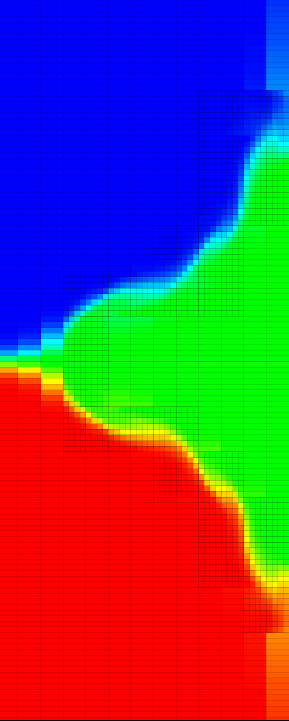
\includegraphics[width=.75\linewidth]{AdvectionCFErrorCropped.png}
  \caption{Without advective refluxing.}
  \label{fig:subWithoutRefluxing}
\end{subfigure}%
\begin{subfigure}{.5\textwidth}
  \centering
  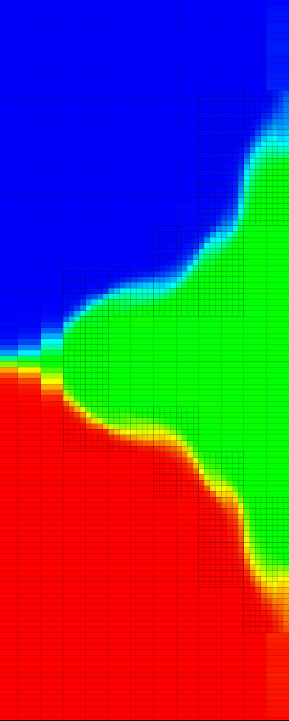
\includegraphics[width=.75\linewidth]{AdvectiveRefluxFixCropped.png}
  \caption{With advective refluxing.}
  \label{fig:subWithRefluxing}
\end{subfigure}
\caption{The effect of refluxing. Notice the error that is building up at the CF interface along the right boundary of figure \ref{fig:subWithoutRefluxing}. This is non-physical and points to a violated conservation law. Advective refluxing during level synchronization largely reduces these errors as can be seen in figure \ref{fig:subWithRefluxing}. \hilight{TODO: Make this greyscale and add a legend.}}
\label{fig:AdvectiveRefluxingEffect}
\end{figure}

\subsection{Adding topography}
In section \ref{NewIBCSetup}, we saw that setting up a customized IBC class involved $3$ steps:
\begin{enumerate}
  \item Creating a child of \texttt{PhysBCUtil} and overriding certain functions.
  \item Assigning an integer to your new class that can be used by the input files.
  \item Telling whoever constructs new \texttt{PhysBCUtil}s about your new child.
\end{enumerate}
Creating your own topography follows the same procedure, except the class structure is slightly different (see figure \ref{fig:MappingClassDia}). Every mapping class you will ever create inherits from \texttt{GeoSourceInterface}. At a minimum, you can create a new coordinate map by creating a child class of \texttt{GeoSourceInterface} and overriding the \texttt{fill\_physCoor} function to produce $x^{\alpha}(\xi^i)$. The parent \texttt{GeoSourceInterface} will then use the child's \texttt{fill\_physCoor} to construct all other geometric quantities needed by the AMR solver such as the Jacobian and metric tensor.\\

\begin{figure}
\centering
\tikzstyle{abstract}=[rectangle, draw=black, rounded corners, fill=blue!40, drop shadow,
        text centered, anchor=north, text=black, text width=4cm]
\tikzstyle{comment}=[rectangle, draw=black, rounded corners, fill=green, drop shadow,
        text centered, anchor=north, text=white, text width=3cm]
\tikzstyle{myarrow}=[->, >=triangle 90, thick]
\tikzstyle{line}=[-, thick]
\begin{tikzpicture}[every node/.style={scale=0.8}]
	\node (GeoSourceInterface) [abstract, text width=4.1cm]
	{\textbf{GeoSourceInterface}};

	\node (auxNode00) [right=0.5cm of GeoSourceInterface] {};
    \draw[myarrow] (auxNode00.center) to (GeoSourceInterface.east);

	% Begin 2nd column
	\node (auxNode01) [right=2.0cm of auxNode00] {};

	\node (CylindricalMap) [abstract, above=0.05cm of auxNode01, text width=3.5cm]
	{\textbf{CylindricalMap}};
    \draw[line] (CylindricalMap.west) -- ++(0,0) -| (auxNode00.center);

	\node (CartesianMap) [abstract, above=0.3cm of CylindricalMap, text width=3.1cm]
	{\textbf{CartesianMap}};
    \draw[line] (CartesianMap.west) -- ++(0,0) -| (auxNode00.center);

	\node (TwistedMap) [abstract, below=0.05cm of auxNode01, text width=2.6cm]
	{\textbf{TwistedMap}};
    \draw[line] (TwistedMap.west) -- ++(0,0) -| (auxNode00.center);

	\node (BathymetricBaseMap) [abstract, below=0.3cm of TwistedMap, text width=4.6cm]
	{\textbf{BathymetricBaseMap}};
    \draw[line] (BathymetricBaseMap.west) -- ++(0,0) -| (auxNode00.center);

	\node (auxNode10) [right=0.5cm of BathymetricBaseMap] {};
    \draw[myarrow] (auxNode10.center) to (BathymetricBaseMap.east);

	% Begin 3rd column
	\node (BeamGenerationMap) [abstract, right=0.2cm of auxNode10, text width=4.5cm]
	{\textbf{BeamGenerationMap}};
    \draw[line] (BeamGenerationMap.west) -- ++(0,0) -| (auxNode10.center);

	\node (LedgeMap) [abstract, above=0.3cm of BeamGenerationMap, text width=2.5cm]
	{\textbf{LedgeMap}};
    \draw[line] (LedgeMap.west) -- ++(0,0) -| (auxNode10.center);
\end{tikzpicture}
\caption{Inheritance diagram of the coordinate mapping system.}
\label{fig:MappingClassDia}
\end{figure}

Most of the time, we are only interested in creating a terrain-following coordinate system. Specifying all three functions, $x^{\alpha}(\xi^i)$, throughout the entire domain is unnecessary -- we really only need to specify the elevation of the ocean bottom at each point in the horizontal domain, $h(x,y)$. For this purpose, we can instead create a child of \texttt{BathymetricBaseMap} and override the \texttt{fill\_bathymetry} function.
%An example of this is the \texttt{BeamGenerationMap} class used to create the submarine ridge of figure \ref{fig:uBeams}.
Creating a terrain-following coordinate system via \texttt{BathymetricBaseMap} will be the focus of the rest of this section.

\begin{lstlisting}[caption={The \texttt{LedgeMap} class header.},label=lstLedgeMapH]
/*************************************************************************
 *    FILE: LedgeMap.H
 *    DESC: A submarine ledge with a smooth, cubic transition region.
 *    DATE: Fri 07 Feb 2014 01:01:34 PM EST
 *    MAIL: santilli@physics.unc.edu
 ************************************************************************/
#ifndef __LedgeMap_H__INCLUDED__
#define __LedgeMap_H__INCLUDED__

#include "BathymetricBaseMap.H"


class LedgeMap: public BathymetricBaseMap
{
public:
    // Constructor
    LedgeMap ();

    // Must return the name of the coordinate mapping
    virtual const char* getCoorMapName () const;

    // Must return whether or not this metric is diagonal
    virtual bool isDiagonal () const;

protected:
    // Fills a NodeFAB with the bathymetric data. a_dest must be flat in
    // the vertical. Upon return, each point in the horizontal (Xi,Eta)
    // of a_dest will contain the elevation.
    // NOTE: This elevation is measured in along the Cartesian vertical
    // coordinate line -- opposite to the direction of gravity.
    virtual void fill_bathymetry (FArrayBox&       a_dest,
                                  const int        a_destComp,
                                  const FArrayBox& a_cartPos,
                                  const RealVect&  a_dXi) const;

	// Member variables
    int m_transitionOrder;
    Real m_hl, m_hr, m_xl, m_xr;
    Real m_coeff0, m_coeff1, m_coeff2, m_coeff3;
};


#endif //!__LedgeMap_H__INCLUDED__
\end{lstlisting}

Listing \ref{lstLedgeMapH} shows the code that we need to write. The constructor will set up the member variables and the \texttt{fill\_bathymetry} function will be the workhorse. The remaining two functions are trivial and can be inlined if desired.\\

As a first version, we will make the constructor do nothing and the \texttt{fill\_bathymetry} function will simply create two regions of distinct elevation separated by a linear transition region (figure \ref{fig:LedgeMapICLinear}).\\

\begin{lstlisting}[caption={Our first version of the \texttt{fill\_bathymetry} function. This will provide a linear transition region. All geometric parameters are hard-coded.},float=h]
	// The geometric parameters.
	// NOTE: This is just for instructional purposes. Hard coded values
	// should always be avoided! We will fix this in the next section.
	m_hl = 0.3; // The left ledge elevation
	m_hr = 0.0; // The right ledge elevation
    m_xl = 2.0; // The x-coor of the left side of the transition.
    m_xr = 3.0; // The x-coor of the right side of the transition.

    Real dh = m_hl - m_hr;
    Real dx = m_xl - m_xr;
	m_coeff0 = m_hr - m_xr*dh/dx;
	m_coeff1 = dh/dx;

	// Loop over the grid and set the bottom elevation.
	// NOTE: a_dest.box() was defined in BathymetricBaseMap to be
	// node-centered and flat in the vertical.
    Real x;
    BoxIterator bit(a_dest.box());
	for (bit.reset(); bit.ok(); ++bit) {
		const IntVect& iv = bit();
		x = a_cartPos(iv, 0);

		if (x < m_xl) {
			a_dest(iv,a_destComp) = m_hl;
		} else if (x > m_xr) {
			a_dest(iv,a_destComp) = m_hr;
		} else {
			a_dest(iv,a_destComp) = m_coeff0 + x*m_coeff1;
		}
	}
\end{lstlisting}

\begin{figure}
\centering
\begin{subfigure}{\textwidth}
  \centering
  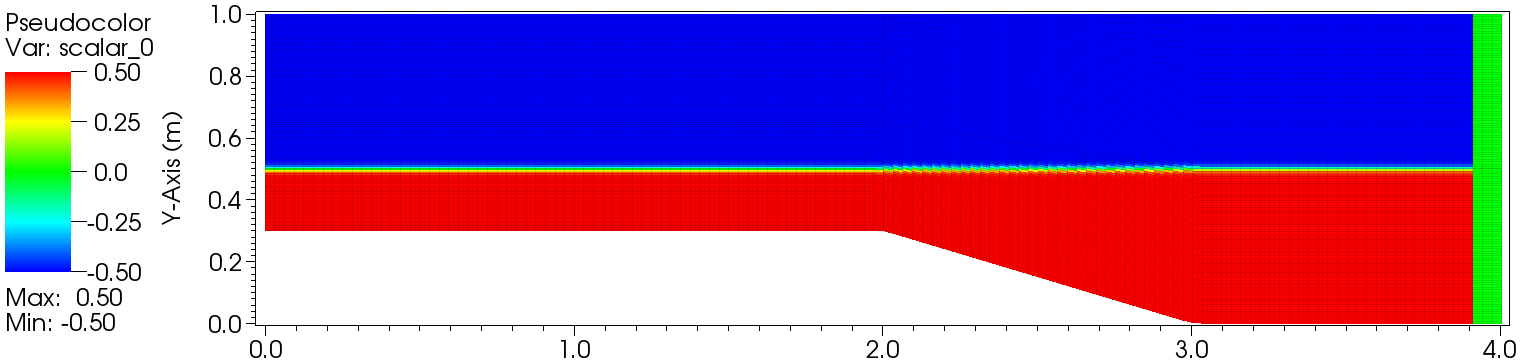
\includegraphics[width=\textwidth]{LedgeMap_ICLinear.png}
  \caption{}
  \label{fig:LedgeMapICLinear}
\end{subfigure}
\\
\begin{subfigure}{\textwidth}
  \centering
  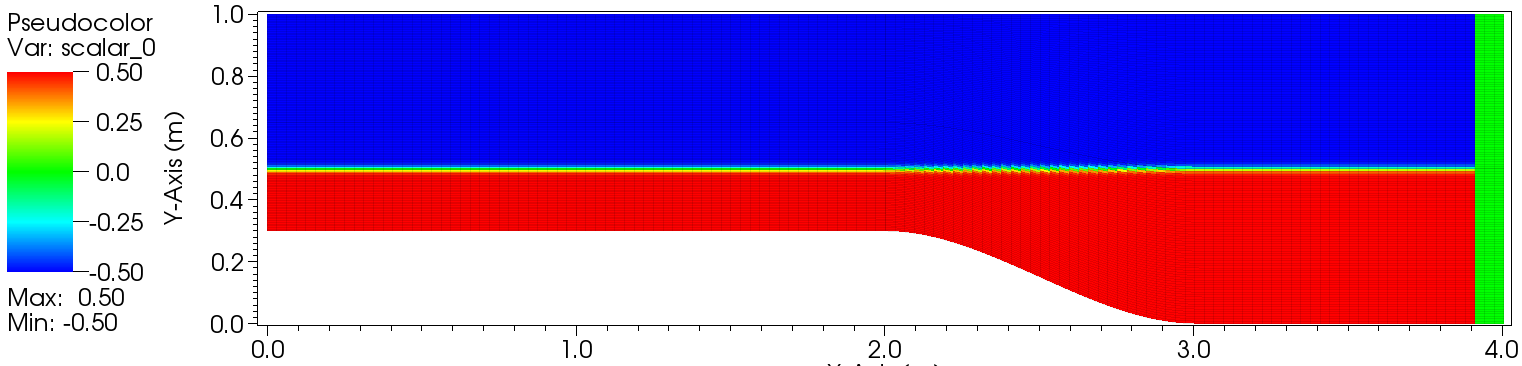
\includegraphics[width=\textwidth]{LedgeMap_ICCubic.png}
  \caption{}
  \label{fig:LedgeMapICCubic}
\end{subfigure}
\caption{The initial buoyancy field in a geometry with (\ref{fig:LedgeMapICLinear}) a linear transition region and (\ref{fig:LedgeMapICCubic}) a cubic transition region.}
\label{fig:LedgeMapICs}
\end{figure}

Once this code compiles, you need to register your new mapping class with the \texttt{CoordMap} enumeration in \texttt{ProblemContext.H}. Then, you must open the \texttt{newGeoSourceInterface} function in the \texttt{ProblemContext.cpp} file and add a \texttt{case} to the \texttt{switch} block that creates your new map. This process is extremely similar to what we have done in the \texttt{InternalWaveBCUtil} example and is left to the reader. Once completed, you should be able to run your simulation and watch the internal wave travel across the ledge.\\

Although this code works just fine, there are some points that need to be addressed. First of all, we hard-coded the geometric parameters. This is clearly bad programming practice because we will have to remember to change these values and recompile every time we change the geometric parameters in the input file. The proper way to obtain these values is by reading them from the input file along with all other geometric parameters. This will be the focus of section \ref{HowToReadFromTheInputFile}.\\

Another point worth mentioning is that we are re-calculating the exact same linear coefficients every time this function is called. In this case, we may not see much of a performance impact because the coefficients are so cheap to compute, but what if we had a more complex geometry? Or worse -- what if we were reading the ledge elevations from an input file? Although the AMR code is smart enough to cache commonly used metrics, this function will still be called quite a bit and we should do our best to optimize it. Luckily, there is an easy fix -- move the repetitive computation to the constructor.\\

Once the coefficient calculations are moved to the constructor, we can create more complex geometries with minimal performance impact. For example, we can smooth-out the transition region with a cubic spline. You should try this for yourself (without looking at the final version of the code). For convenience, here are the cubic's coefficients.
\begin{align*}
	c_0 &= h_r + x_r^2 (h_l-h_r) (3x_l-x_r) / (x_l-x_r)^3\\
	c_1 &= -6 x_l x_r (h_l-h_r) / (x_l-x_r)^3\\
	c_2 &= 3 (x_l+x_r) (h_l-h_r) / (x_l-x_r)^3\\
	c_3 &= -2 (h_l-h_r) / (x_l-x_r)^3
\end{align*}
Here, $c_i$ is the coefficient of the $i^{th}$ power of $x$ and each parameter is easily identified with its coded version (e.g. $h_l$ $\leftrightarrow$ \texttt{m\_hl}). Figure \ref{fig:LedgeMapICCubic} shows what this cubic transition region should look like.

\subsection{Reading the input file}\label{HowToReadFromTheInputFile}
You may have noticed that Chombo includes a nice class called \texttt{ParmParse}. This does not just blindly read data from a text file, but actually parses it, as the name suggests. This allows the input file to contain comments and an arbitrary amount of whitespace, which helps make the input file human-readable. \texttt{ParmParse} also allows the code to not just ask for parameters, but ask whether parameters were provided at all. It also asks for prefixes on all of the input parameters, which gives each part of code its own namespace. This prevents a clash if, say, the AMR projector and the LES both need a parameter called \texttt{numiters}. I highly suggest that all portions of the code read from a single input file that completely defines the simulation.\\

All of the operations that read from the input file are in one place -- the \texttt{ProblemContext} class. This class follows what is called a \textit{singleton} design pattern. A singleton is a class whose constructor is guaranteed to be called only once throughout the simulation. By placing all read operations in its constructor, we can ask \texttt{ProblemContext} for input parameters anywhere in our code without the risk of slow and repetitive IO and parsing. (\textit{Note:} To facilitate its ease of use, the public members of this class do not have the standard \texttt{m\_} prefix. This is the only class that ignores this standard.) I suggest that you read about the \texttt{ParmParse} functionality, which is documented in Chombo's online reference manual\footnote{\url{http://davis.lbl.gov/Manuals/CHOMBO-RELEASE-3.1/classes.html}}. Then, take a look at the \texttt{ProblemContext} code, which is in the \texttt{utils} directory, and become familiar with its organization and functionality.\\

In this section, we will add five parameters to the input file as shown in listing \ref{lstLedgeMapInputParams}. To do so is not difficult. We first create five public member variables in \texttt{ProblemContext} that will hold the values, then we place five calls to \texttt{ParmParse} to read the values from disk. That's it! We will then be able to ask for these parameters anywhere we like -- including the constructor of our \texttt{LedgeMap} class. At this point, I will not describe every step, but instead just provide the solution. If help is needed, you can use the Chombo design document and online reference manual to learn how each line works.

\begin{lstlisting}[caption={The five new input parameters that describe the ledge.},label=lstLedgeMapInputParams]
geometry.ledgeMapTransitionOrder = 1
geometry.ledgeMapHl = 0.3
geometry.ledgeMapHr = 0.0
geometry.ledgeMapXl = 2.0
geometry.ledgeMapXr = 3.0
\end{lstlisting}

\begin{lstlisting}[caption={\texttt{ProblemContext}'s new member variables. This should be placed in the public block under the \texttt{readGeometry()} declaration in \texttt{ProblemContext.H}.}]
	// Parameters specific to LedgeMap
	int ledgeMapTransitionOrder;
	Real ledgeMapHl;
	Real ledgeMapHr;
	Real ledgeMapXl;
	Real ledgeMapXr;
\end{lstlisting}

\begin{lstlisting}[caption={This actually performs the IO and should be placed in the \texttt{readGeometry()} function of \texttt{ProblemContext.cpp}.}]
	switch (coordMap) {
	case CoordMap::LEDGE:
		ppGeo.get("ledgeMapTransitionOrder", ledgeMapTransitionOrder);
		pout() << "\tledgeMapTransitionOrder = "
			   << ledgeMapTransitionOrder << endl;

		ppGeo.get("ledgeMapHl", ledgeMapHl);
		pout() << "\tledgeMapHl = " << ledgeMapHl << endl;

		ppGeo.get("ledgeMapHr", ledgeMapHr);
		pout() << "\tledgeMapHr = " << ledgeMapHr << endl;

		ppGeo.get("ledgeMapXl", ledgeMapXl);
		pout() << "\tledgeMapXl = " << ledgeMapXl << endl;

		ppGeo.get("ledgeMapXr", ledgeMapXr);
		pout() << "\tledgeMapXr = " << ledgeMapXr << endl;

		break;

	case ...
		// Code for other coordinate maps.
    }
\end{lstlisting}

\begin{lstlisting}[caption={The new \texttt{LedgeMap} constructor.}]
// -----------------------------------------------------------------------
// Constructor
// -----------------------------------------------------------------------
LedgeMap::LedgeMap ()
: BathymetricBaseMap()
{
	// Obtain a pointer to the one-and-only ProblemContext object.
    const ProblemContext* ctx = ProblemContext::getInstance();

	// Collect the needed parameters.
    m_transitionOrder = ctx->ledgeMapTransitionOrder;
    m_hl = ctx->ledgeMapHl;
    m_hr = ctx->ledgeMapHr;
    m_xl = ctx->ledgeMapXl;
    m_xr = ctx->ledgeMapXr;

	// Compute the coefficients.
    Real dh = m_hl - m_hr;
    Real dx = m_xl - m_xr;
    Real invdx3 = pow(dx, -3.0);

    if (m_transitionOrder == 1) {
        // Linear transition
        m_coeff0 = m_hr - m_xr*dh/dx;
        m_coeff1 = dh/dx;
        m_coeff2 = 0.0;
        m_coeff3 = 0.0;
    } else if (m_transitionOrder == 3) {
        // Cubic transition
        m_coeff0 = m_hr + dh*(3.0*m_xl-m_xr)*m_xr*m_xr*invdx3;
        m_coeff1 = -6.0*dh*m_xl*m_xr*invdx3;
        m_coeff2 = 3.0*dh*(m_xl+m_xr)*invdx3;
        m_coeff3 = -2.0*dh*invdx3;
    } else {
        MayDay::Error("LedgeMap::m_transitionOrder must be 1 or 3");
    }
}
\end{lstlisting}

\begin{lstlisting}[caption={The updated \texttt{fill\_bathymetry} function. Notice that this code checks if \texttt{a\_dest} is properly defined. These checks will only exist in debug mode. If desired, the for-loop can be implemented and optimized in Fortran, but I will leave that to the reader.}]
// -----------------------------------------------------------------------
// Fills a NodeFAB with the bathymetric data. a_dest must be flat in the
// vertical. Upon return, each point in the horizontal (Xi,Eta) of a_dest
// will contain the (positive) local depth.
// NOTE: This vertical distance is measured in a straight line perp
// to the surface. We are measuring this distance along the Cartesian
// vertical coordinate line, not the mapped vertical coordinate line.
// -----------------------------------------------------------------------
void LedgeMap::fill_bathymetry (FArrayBox&       a_dest,
                                const int        a_destComp,
                                const FArrayBox& a_cartPos,
                                const RealVect&  a_dXi) const
{
    const Box& destBox = a_dest.box();
    const IntVect destBoxType = destBox.type();
    BoxIterator bit(destBox);
    Real x;

    // The holder needs to be flat and nodal in the vertical.
    CH_assert(destBox == horizontalDataBox(destBox));
    CH_assert(destBoxType[SpaceDim-1] == 1);

	for (bit.reset(); bit.ok(); ++bit) {
		const IntVect& iv = bit();
		x = a_cartPos(iv, 0);

		if (x < m_xl) {
			a_dest(iv,a_destComp) = m_hl;
		} else if (x > m_xr) {
			a_dest(iv,a_destComp) = m_hr;
		} else {
			a_dest(iv,a_destComp) = m_coeff0 + x*(m_coeff1 + x*(m_coeff2 + x*m_coeff3));
		}
	}
}
\end{lstlisting}

\subsection{Adding tidal forcing and sponges}

At this point, you should be quite familiar with the way the code is organized and how BoxTools is used, so turning on the tidal forcing and sponges should be rather simple. Consider the input parameters shown in listing \ref{lstTidalSpongeParams}.
\begin{lstlisting}[label=lstTidalSpongeParams,caption={Sample tidal and sponge forcing input parameters.}]
  ### tidal parameters
  ibc.tidalOmega = 0.0001407
  ibc.tidalU0 = 0.01407

  ### Sponge layer parameters
  ibc.useSpongeLayer = 1
  ibc.spongeWidthLo = 0.12 0.0
  ibc.spongeWidthHi = 0.12 0.0
  # ibc.spongeWidthFracLo = 0.08 0.00
  # ibc.spongeWidthFracHi = 0.08 0.00
  ibc.spongeDtMultLo = 15.0 15.0
  ibc.spongeDtMultHi = 15.0 15.0  
\end{lstlisting}
The first two parameters set the tidal frequency ($rad/s$) and maximum tidal speed. If these parameters are non-zero and present in the input file, then tidal forcing will be used. The rest of the parameters control the sponge sizes and strengths. \texttt{spongeWidthLo} is a vector specifying the absolute thickness of the sponges in each direction on the lower faces of the domain while \texttt{spongeWidthHi} does the same for the upper faces. The \texttt{spongeWidthFrac*} parameters are similar, but they specify fractions of the domain lengths in each direction rather than absolute lengths. For example, the \texttt{spongeWidthFrac*} parameters shown in listing \ref{lstTidalSpongeParams} would create sponges in the x-direction that each span $8\%$ of the domain, if they hadn't been commented out. If you choose to provide \texttt{spongeWidthFrac*}, then you must not provide \texttt{spongeWidth*}.\\

If you decide to use a sponge, you must also specify what the target velocity and scalar values will be. To do this, you must override two \texttt{PhysBCUtil} functions, \texttt{fillVelSpongeLayerTarget} and \texttt{fillScalarSpongeLayerTarget}. By default, these functions throw an error and halt execution.

% 
%\appendix
%\input{./tex/myappendix.tex}
% 
% 
%%% Bibliography:
%\clearpage
\bibliographystyle{ieeetr}
\bibliography{./bibliography}

\end{document}

